\section{Summary of Paper \ref{pap:physics}}
\subsection*{"\nameref{pap:physics}"}
\subsection*{Scope and Motivations}
It was shown in Paper \ref{pap:pit} that it is possible to identify a model from calm water free running model test with inverse dynamics regression (\autoref{sec:IDR}) together with a cross validation technique (\autoref{sec:cross_validation}) to unsure good generalization (\autoref{sec:generalization}) so that the model can predict other kinds of maneuvers with very good accuracy. It was however soon discovered that these models did not generalize well when wind forces were added to the simulations. This problem was addressed in Paper \ref{pap:physics}.

Paper \ref{pap:physics} uses two modular manoeuvring models: PI and PU. They have identical prediction models for the hull and propeller forces but different models for the rudder forces. The PI model has a new deterministic semi-empirical rudder model, as proposed the paper. The PU model has a data-driven mathematical rudder model. Except for the changed rudder models, the ship manoeuvring models are similar to the MMG model \cite{yasukawa_introduction_2015}, with some minor enhancements; The surge velocity is for instance expressed as a perturbed velocity (see \autoref{sec:prime_system}) allowing for higher order resistance coefficients.

A brief description of the workflow of Paper \ref{pap:physics} is shown in \autoref{fig:methodology}.
The PI and PU models are identified on free running model tests via inverse dynamics and regression. To assess the physical correctness, a reference model is established, where the PI model is instead identified on a VCT dataset. This reference model, based on CFD, is assumed to be a sufficiently correct representation of the ship's physics.
Verification and comparisons between the models are carried out on the free sailing model tests.
\begin{figure}[h]
  \centering
  %\includesvg[width=\columnwidth, pretex=\scriptsize, height=12cm]{figures/methodology2.svg}
  \includesvg[pretex=\centering\fontsize{7.5}{8}]{kappa/images/methodology2.svg}
  \caption{Research workflow, describing how the reference model is identified with regression of VCT data and the PI and PU models are identified with regression of inverse dynamics forces from model tests. Results are then gathered to assess the parameter drift, physical correctness and generalization of the models.}
  \label{fig:methodology}
\end{figure}
It was investigated if the introduction of a deterministic semi-empirical rudder model in the PI model would reduce the multicollinearity and enhance the generalization.

\FloatBarrier
\subsection*{Results and Conclusions}

\begin{figure}[h]
    \centering
    \includegraphics{kappa/images/results.ID_zigzag10.pdf}
    \caption{ID estimations of $Y_D$ and $N_D$ during a zigzag10/10 model test compared with model predictions.}
    \label{fig:ID_zigzag10}
\end{figure}

\begin{figure}[h]
    \begin{center}
        \includesvg{kappa/images/results.hull_force_decomposition_zigzag20.svg}
        \caption{Decomposition of hull forces and moments during a zigzag20/20 test for parameters related to drift, yaw rate the prediction models.}
        \label{fig:ID_regression_N_decomposition}
    \end{center}
\end{figure}

\begin{figure}[h!]
    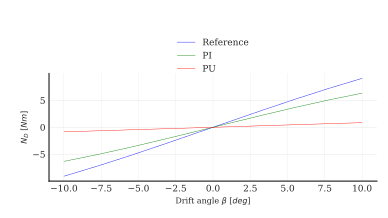
\includegraphics{kappa/images/result_wind_state.forces.pdf}
    \caption{Total sway force and yawing moment from the wPCC models at various drift angles.}
    \label{fig:result_wind_state}
\end{figure}

\subsection*{Comments}
\clearpage